\chapter{story of a beep}
\label{sec:cursor_crossed_a_line}
\lhead[tempest]{}
\lstset{style=6502Style}
Whenever the cursor is moved left or right, \textit{Tempest} emits a beep. This is the story of that
beep. To tell the story we will start at the end rather than the beginning.

To magic up this beep, we have to emit a series of commands to the Atari cabinet's sound chip, known
as the \icode{POKEY}. These commands are as follows:

\begin{figure}[H]
  {
    \setlength{\tabcolsep}{3.0pt}
    \setlength\cmidrulewidth{\heavyrulewidth} % Make cmidrule = 
    \begin{adjustbox}{width=12.5cm,center}
      \begin{tabular}{lllll}
        \toprule
        Register & Description & Value & Bits & Meaning\\
        \midrule
        \icode{AUDC1} & Channel 1 Control & \icode{A2} &\icode{10110010} & Rectangular curve, volume 2\\
        \icode{AUDF1} & Channel 1 Frequency & \icode{0F} &\icode{00001111} & High pitched sound\\
        \addlinespace
        \bottomrule
      \end{tabular}
    \end{adjustbox}
  }
\end{figure}

Then after a short interval, we follow up with the commands to stop the sound:
\begin{figure}[H]
  {
    \setlength{\tabcolsep}{3.0pt}
    \setlength\cmidrulewidth{\heavyrulewidth} % Make cmidrule = 
    \begin{adjustbox}{width=9.5cm,center}
      \begin{tabular}{lllll}
        \toprule
        Register & Description & Value & Bits & Meaning\\
        \midrule
        \icode{AUDC1} & Channel 1 Control & \icode{00} &\icode{00000000} & Stop\\
        \icode{AUDF1} & Channel 1 Frequency & \icode{00} &\icode{00000000} & No sound\\
        \addlinespace
        \bottomrule
      \end{tabular}
    \end{adjustbox}
  }
\end{figure}

It's as simple as that. But since we will want to generate more complex sounds later, we
have to develop some machinery that's capable of emitting more than just a single beep.
So it will be instructive, with this minimally simple example, to see how this machinery
generates the above commands, which consist of little more than telling the sound chip
to play a beep and then stop. We find our sound definitions and the machinery underlying
them in \icode{ALSOUN.MAC}.

So below is the data driving our 'cursor crossing a line' beep. There are two sequences of bytes.
The first defines the values and the timing for writing those values to the \icode{AUDF1}
register. Writing something to \icode{AUDF1} is like playing a note. The value we write 
determines the note that will be played.

The second sequence defines the way that note is played. We can manipulate the performance
of the note by writing to the \icode{AUDC1} register. Depending on the value we write we
can alter the volume and the distortion applied to the note we selected.

\begin{lstlisting}
LO5F:   .BYTE 0F,4,0,1   ; CURSOR CROSSED A LINE
        .BYTE 0,0
LO5A:   .BYTE 0A2,4,40,1
        .BYTE 0,0
\end{lstlisting}

It will be easier to understand the above sequence definition if we comment the purpose
of each byte in the sequence:
\begin{lstlisting}
LO5F:   .BYTE 0F  ; VALUE TO WRITE TO AUDF1
        .BYTE 4   ; BEATS TO WAIT BEFORE NEXT CHANGE
        .BYTE 0   ; AMOUNT TO CHANGE BY
        .BYTE 1   ; NUMBER OF TIMES TO CHANGE (1 MEANS 0)
        .BYTE 0   ; RESTART POSITION (0 MEANS NO RESTART) 
        .BYTE 0   ; STOP

LO5A:   .BYTE 0A2 ; VALUE TO WRITE TO AUDC1
        .BYTE 4   ; BEATS TO WAIT BEFORE NEXT CHANGE
        .BYTE 40  ; AMOUNT TO CHANGE BY
        .BYTE 1   ; NUMBER OF TIMES TO CHANGE (1 MEANS 0)
        .BYTE 0   ; RESTART POSITION (0 MEANS NO RESTART) 
        .BYTE 0   ; STOP
\end{lstlisting}

Close inspection of the above example shows that the commands we set out on the previous page
are the result of following the instructions of each of these byte sequences. For the \icode{LO5F}
sequence, which controls what we write to the \icode{AUDF1} register, we write the following commands
to turn on the note, wait 4 frames, and then turn it off again:

\begin{figure}[H]
  {
    \setlength{\tabcolsep}{3.0pt}
    \setlength\cmidrulewidth{\heavyrulewidth} % Make cmidrule = 
    \begin{adjustbox}{width=12.5cm,center}
      \begin{tabular}{lllll}
        \toprule
        Register & Description & Value & Bits & Meaning\\
        \midrule
        \icode{AUDF1} & Channel 1 Frequency & \icode{0F} &\icode{00001111} & High pitched sound\\
        \icode{AUDF1} & Channel 1 Frequency & \icode{00} &\icode{00000000} & No sound\\
        \addlinespace
        \bottomrule
      \end{tabular}
    \end{adjustbox}
  }
\end{figure}

\begin{figure}[H]
{
    \begin{subfigure}{0.23\textwidth}
      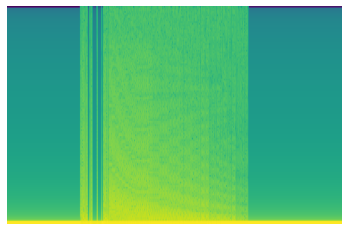
\includegraphics[width=3cm]{tempest_sounds/buttons/CPEXPL.raw-button.png}%
      \makebox[0pt][r]{%
        \raisebox{.3cm}{%
          \textattachfile{src/tempest_sounds/wav/CPEXPL.raw.wav}{
\includegraphics[width=1.5cm]{sounds/play.png}}%
        }\hspace*{0.75cm}%
      }%
      \caption*{CPEXPL}
    \end{subfigure}
    \begin{subfigure}{0.23\textwidth}
      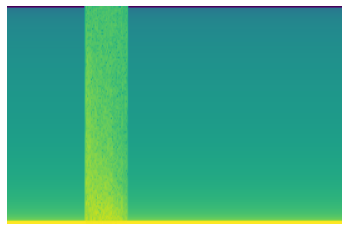
\includegraphics[width=3cm]{tempest_sounds/buttons/ESLSON.raw-button.png}%
      \makebox[0pt][r]{%
        \raisebox{.3cm}{%
          \textattachfile{src/tempest_sounds/wav/ESLSON.raw.wav}{
\includegraphics[width=1.5cm]{sounds/play.png}}%
        }\hspace*{0.75cm}%
      }%
      \caption*{ESLSON}
    \end{subfigure}
    \begin{subfigure}{0.23\textwidth}
      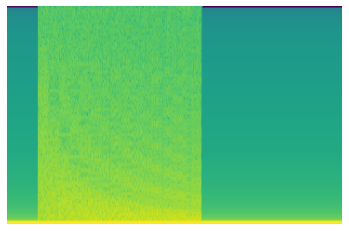
\includegraphics[width=3cm]{tempest_sounds/buttons/EXSNON.raw-button.png}%
      \makebox[0pt][r]{%
        \raisebox{.3cm}{%
          \textattachfile{src/tempest_sounds/wav/EXSNON.raw.wav}{
\includegraphics[width=1.5cm]{sounds/play.png}}%
        }\hspace*{0.75cm}%
      }%
      \caption*{EXSNON}
    \end{subfigure}
    \begin{subfigure}{0.23\textwidth}
      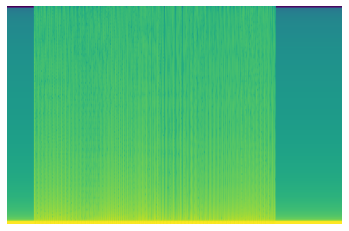
\includegraphics[width=3cm]{tempest_sounds/buttons/PULSTR.raw-button.png}%
      \makebox[0pt][r]{%
        \raisebox{.3cm}{%
          \textattachfile{src/tempest_sounds/wav/PULSTR.raw.wav}{
\includegraphics[width=1.5cm]{sounds/play.png}}%
        }\hspace*{0.75cm}%
      }%
      \caption*{PULSTR}
    \end{subfigure}
    \begin{subfigure}{0.23\textwidth}
      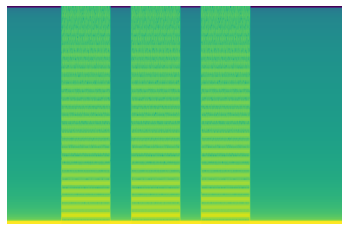
\includegraphics[width=3cm]{tempest_sounds/buttons/S3SWAR.raw-button.png}%
      \makebox[0pt][r]{%
        \raisebox{.3cm}{%
          \textattachfile{src/tempest_sounds/wav/S3SWAR.raw.wav}{
\includegraphics[width=1.5cm]{sounds/play.png}}%
        }\hspace*{0.75cm}%
      }%
      \caption*{S3SWAR}
    \end{subfigure}
    \begin{subfigure}{0.23\textwidth}
      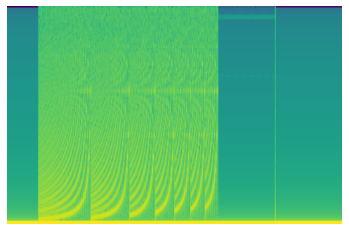
\includegraphics[width=3cm]{tempest_sounds/buttons/SAUSON.raw-button.png}%
      \makebox[0pt][r]{%
        \raisebox{.3cm}{%
          \textattachfile{src/tempest_sounds/wav/SAUSON.raw.wav}{
\includegraphics[width=1.5cm]{sounds/play.png}}%
        }\hspace*{0.75cm}%
      }%
      \caption*{SAUSON}
    \end{subfigure}
    \begin{subfigure}{0.23\textwidth}
      
\includegraphics[width=3cm]{tempest_sounds/buttons/SBOING.raw-button.png}%
      \makebox[0pt][r]{%
        \raisebox{.3cm}{%
          \textattachfile{src/tempest_sounds/wav/SBOING.raw.wav}{
\includegraphics[width=1.5cm]{sounds/play.png}}%
        }\hspace*{0.75cm}%
      }%
      \caption*{SBOING}
    \end{subfigure}
    \begin{subfigure}{0.23\textwidth}
      
\includegraphics[width=3cm]{tempest_sounds/buttons/SELICO.raw-button.png}%
      \makebox[0pt][r]{%
        \raisebox{.3cm}{%
          \textattachfile{src/tempest_sounds/wav/SELICO.raw.wav}{
\includegraphics[width=1.5cm]{sounds/play.png}}%
        }\hspace*{0.75cm}%
      }%
      \caption*{SELICO}
    \end{subfigure}
    \begin{subfigure}{0.245\textwidth}
      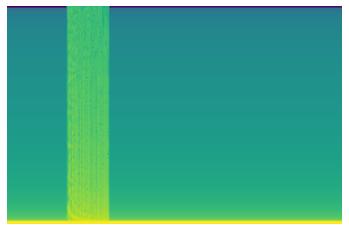
\includegraphics[width=3cm]{tempest_sounds/buttons/SLAUNC.raw-button.png}%
      \makebox[0pt][r]{%
        \raisebox{.3cm}{%
          \textattachfile{src/tempest_sounds/wav/SLAUNC.raw.wav}{
\includegraphics[width=1.5cm]{sounds/play.png}}%
        }\hspace*{0.75cm}%
      }%
      \caption*{SLAUNC}
    \end{subfigure}
    \begin{subfigure}{0.245\textwidth}
      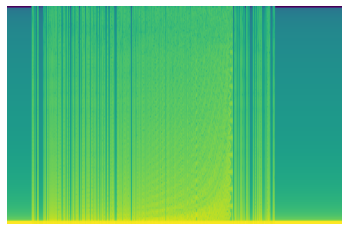
\includegraphics[width=3cm]{tempest_sounds/buttons/SOUTS2.raw-button.png}%
      \makebox[0pt][r]{%
        \raisebox{.3cm}{%
          \textattachfile{src/tempest_sounds/wav/SOUTS2.raw.wav}{
\includegraphics[width=1.5cm]{sounds/play.png}}%
        }\hspace*{0.75cm}%
      }%
      \caption*{SOUTS2}
    \end{subfigure}
    \begin{subfigure}{0.245\textwidth}
      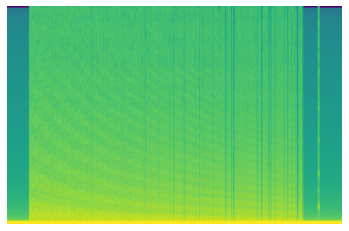
\includegraphics[width=3cm]{tempest_sounds/buttons/SOUTS3.raw-button.png}%
      \makebox[0pt][r]{%
        \raisebox{.3cm}{%
          \textattachfile{src/tempest_sounds/wav/SOUTS3.raw.wav}{
\includegraphics[width=1.5cm]{sounds/play.png}}%
        }\hspace*{0.75cm}%
      }%
      \caption*{SOUTS3}
    \end{subfigure}
    \begin{subfigure}{0.245\textwidth}
      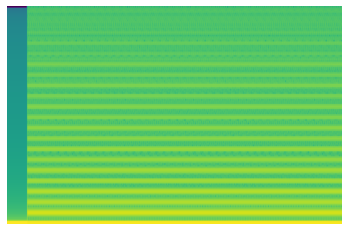
\includegraphics[width=3cm]{tempest_sounds/buttons/SSLAMS.raw-button.png}%
      \makebox[0pt][r]{%
        \raisebox{.3cm}{%
          \textattachfile{src/tempest_sounds/wav/SSLAMS.raw.wav}{
\includegraphics[width=1.5cm]{sounds/play.png}}%
        }\hspace*{0.75cm}%
      }%
      \caption*{SSLAMS}
    \end{subfigure}
}\caption*{All 28 sound samples and their spectrograms. If your reader supports it you can play the samples.}
\end{figure}
Simultaneously the \icode{LO5A} sequence instructs us to set the volume and the sound
type by writing to the \icode{AUDC1} register and then, after 4 frames, silence it again:
\begin{figure}[H]
  {
    \setlength{\tabcolsep}{3.0pt}
    \setlength\cmidrulewidth{\heavyrulewidth} % Make cmidrule = 
    \begin{adjustbox}{width=12.5cm,center}
      \begin{tabular}{lllll}
        \toprule
        Register & Description & Value & Bits & Meaning\\
        \midrule
        \icode{AUDC1} & Channel 1 Control & \icode{A2} &\icode{101,10010} & Rectangular curve, volume 2\\
        \icode{AUDC1} & Channel 1 Control & \icode{00} &\icode{00000000} & Stop\\
        \addlinespace
        \bottomrule
      \end{tabular}
    \end{adjustbox}
  }
\end{figure}

We can look at a slightly more involved example to get an idea of the manipulation that this scheme affords
us. Here are the two sequences that define an 'Enemy Shot' (\icode{ESLSON}):

\begin{lstlisting}
        ; ENEMY SHOT
ES8F:   .BYTE 0   ; VALUE TO WRITE TO AUDF1
        .BYTE 3   ; BEATS TO WAIT BEFORE NEXT CHANGE
        .BYTE 2   ; AMOUNT TO CHANGE BY
        .BYTE 9   ; NUMBER OF TIMES TO CHANGE (1 MEANS 0)
        .BYTE 0   ; RESTART POSITION (0 MEANS NO RESTART) 
        .BYTE 0   ; STOP

ES8A:   .BYTE 8   ; VALUE TO WRITE TO AUDC1
        .BYTE 3   ; BEATS TO WAIT BEFORE NEXT CHANGE
        .BYTE 0FF ; AMOUNT TO CHANGE BY (0FF means -1)
        .BYTE 9   ; NUMBER OF TIMES TO CHANGE (1 MEANS 0)
        .BYTE 0   ; RESTART POSITION (0 MEANS NO RESTART) 
        .BYTE 0   ; STOP
\end{lstlisting}

Notice that the commands are to be run simultaneously: every 3 frames. You can also notice that we are to run
each command 8 times in total (9 - 1). We also note that \icode{0FF} is another way of saying \icode{-1}. So equipped
with these provisions we can execute the commands as follows:

\begin{figure}[H]
  {
    \setlength{\tabcolsep}{3.0pt}
    \setlength\cmidrulewidth{\heavyrulewidth} % Make cmidrule = 
    \begin{adjustbox}{width=11.5cm,center}
      \begin{tabular}{llllll}
        \toprule
        Register & Value & Meaning & Register & Value & Meaning\\
        \midrule
        \icode{AUDC1} &  \icode{08} & Volume 8 & \icode{AUDF1} &  \icode{00} & No Sound\\
        \icode{AUDC1} &  \icode{07} & Volume 7 & \icode{AUDF1} &  \icode{02} & Very Very Low Pitch\\
        \icode{AUDC1} &  \icode{06} & Volume 6 & \icode{AUDF1} &  \icode{04} & Very Low Pitch\\
        \icode{AUDC1} &  \icode{05} & Volume 5 & \icode{AUDF1} &  \icode{06} & Still Low Pitch\\
        \icode{AUDC1} &  \icode{04} & Volume 4 & \icode{AUDF1} &  \icode{08} & Low Pitch\\
        \icode{AUDC1} &  \icode{03} & Volume 3 & \icode{AUDF1} &  \icode{0A} & Getting Higher\\
        \icode{AUDC1} &  \icode{02} & Volume 2 & \icode{AUDF1} &  \icode{0C} & Higher Still\\
        \icode{AUDC1} &  \icode{01} & Volume 1 & \icode{AUDF1} &  \icode{0F} & Higher again\\
        \addlinespace
        \bottomrule
      \end{tabular}
    \end{adjustbox}
  }
\end{figure}

